%%%%%%%%%%%%%%%%%%%%%%%%%%%%%%%%%%%%%%%%%%%%%%%%%%%%%%%%%%
%
% Doctoral Thesis Template @ The University of Manchester
% LaTeX Chapter Template
% Version 1 (23/07/2020)
% Joe Crone
%
% This template is based on:
% The University of Manchester, Presentation of Thesis Policy
% Research Office Graduate Education Team
% June 2017
% http://www.regulations.manchester.ac.uk/pgr-presentation-theses/
%
%%%%%%%%%%%%%%%%%%%%%%%%%%%%%%%%%%%%%%%%%%%%%%%%%%%%%%%%%%
\documentclass[../main.tex]{subfiles}
\begin{document}

% Title
%--------------------------------------------------------
\chapter{Theory of Photon Production by Inverse Compton Scattering}
\label{ChapterTemplate} % to reference use \ref{ChapterTemplate}

\begin{equation}
\frac{\omega'}{\omega} = \gamma\left(1+\beta\cos\theta\right)
\label{eq:doppler_shift}
\end{equation}

\begin{figure}[!htb]
    \centering
    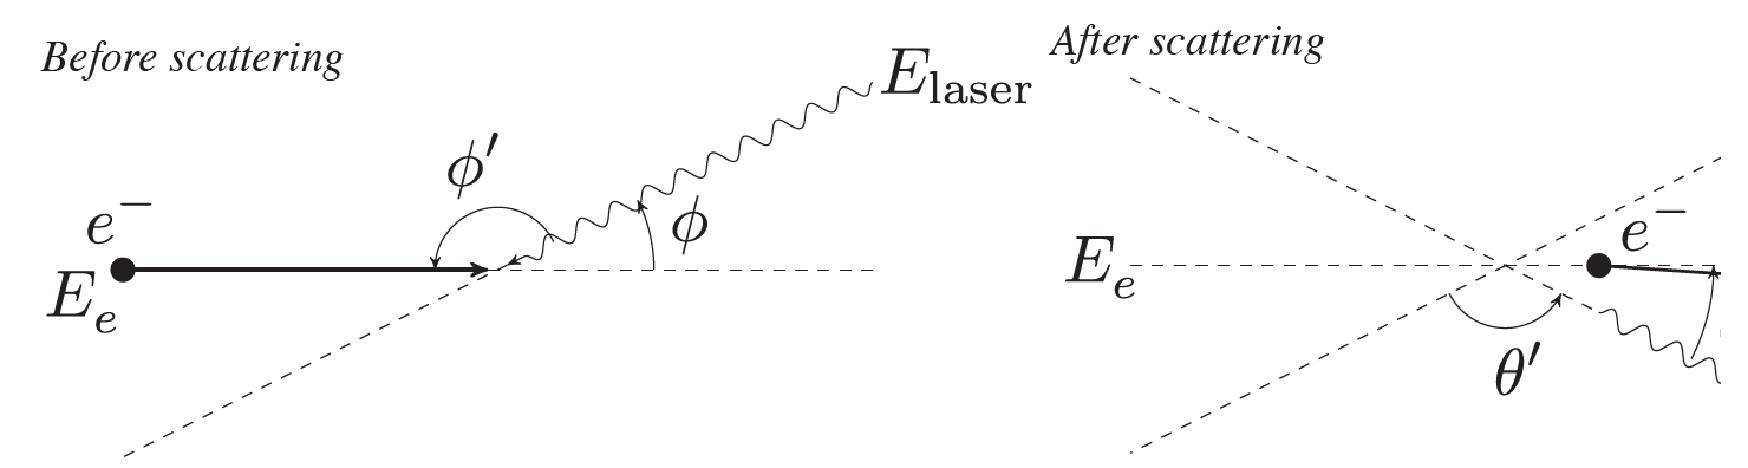
\includegraphics[width=\textwidth]{Figures/scatteringkinematicsdiagram.pdf}
    \caption{Geometry of the inverse Compton scattering event at the interaction point. This geometry follows the geometry prescribed by Sun et al \cite{sun2009energy}. }
    \label{fig:scattered_photon_kinematics}
\end{figure}

\begin{equation}
E_{\gamma} = \frac{\left(1-\beta\cos\phi'\right)E_{L}}{1-\beta\cos\theta+\left(1-\cos\theta'\right)\frac{E_{L}}{E_{e}}} 
\label{eq:scattered_photon_energy}
\end{equation}

In the head-on case, for $\theta \ll 1$ i.e. in the small angle approximation

\begin{equation}
E_{\gamma} \approx \frac{4\gamma^{2}E_{L}}{1+\gamma^{2}\theta^{2}+X}    
\label{eq:small_angle_scattered_photon_energy}
\end{equation}

\begin{equation}
X = \frac{4\gamma E_{L}}{mc^{2}}
\label{eq:recoil_term}
\end{equation}

\end{document}